\documentclass[12pt, twoside]{article}
% \documentclass[12pt, twoside]{article}
\usepackage[letterpaper, margin=1in, headsep=0.2in]{geometry}
\setlength{\headheight}{0.6in}
%\usepackage[english]{babel}
\usepackage[utf8]{inputenc}
\usepackage{microtype}
\usepackage{amsmath}
\usepackage{amssymb}
%\usepackage{amsfonts}
\usepackage[nomessages]{fp} %\FPeval{\var-name}{2*sin(pi/6)}
\usepackage{siunitx} %units in math. eg 20\milli\meter
\usepackage{yhmath} % for arcs, overparenth command
\usepackage{tikz} %graphics
\usetikzlibrary{quotes, angles, arrows, arrows.meta}
\usepackage{graphicx} %consider setting \graphicspath{{images/}}
\usepackage{parskip} %no paragraph indent
\usepackage{enumitem}
\usepackage{multicol}
\usepackage{venndiagram}

\usepackage{fancyhdr}
\pagestyle{fancy}
\fancyhf{}
\renewcommand{\headrulewidth}{0pt} % disable the underline of the header
\raggedbottom
\hfuzz=2mm %suppresses overfull box warnings

\usepackage{hyperref}
\usepackage{float}

\fancyhead[LE]{\thepage}
\fancyhead[RO]{\thepage \\ First and last name: \hspace{2.5cm} \,\\ Section: \hspace{2.5cm} \,}
\fancyhead[LO]{BECA / Dr. Huson / Regents Prep: Graphs\\* 15 November 2024}

\begin{document}

\subsubsection*{3.3 Do Now: Graphing quadratic systems}
\begin{enumerate}
  \item One equation of a system is graphed. Graph the second equation, labeling the intersections as ordered pairs.

  \begin{multicols}{2}
    $y = ax^2 - 2x + 9$ \\
    \columnbreak
    $2x + y = 3$
    \end{multicols}
    Find the value of the leading coefficient $a$ of the quadratic equation. \vspace{2cm}

  \begin{center}
  \begin{tikzpicture}[scale=.635]
    \draw [help lines] (-10,-10) grid (10,10);
    \draw [thick, ->] (-10.2,0) -- (10.4,0) node [below right] {$x$};
    \draw [thick, ->] (0,-10.2)--(0,10.4) node [left] {$y$};
    \draw[thick, <->,smooth, domain=-4.15:2.85] plot (\x, {-1.5*(\x)^2 - 2*\x + 9});
  \end{tikzpicture}
  \end{center}

\newpage
\item Identify the expressions that are equal to $\displaystyle \frac{2^2}{2^4}$
  \begin{multicols}{2}
  \begin{enumerate}
      \item $2^6$
      \item $\displaystyle \frac{1}{2^2}$
      \item $2^{-2}$
      \item $\frac{1}{4}$
      \item $2^{2}$
      \item $0.5$
  \end{enumerate}
  \end{multicols}

\item Identify the expressions that are equal to $\displaystyle 2^{-3}$
  \begin{multicols}{2}
  \begin{enumerate}
      \item $2.333...$
      \item $\sqrt{2}$
      \item $\displaystyle \frac{1}{2^3}$
      \item $\displaystyle \frac{1}{8}$
      \item $6$
      \item $0.125$
  \end{enumerate}
  \end{multicols}

\item Identify the expressions that are equal to $\displaystyle 9^{\frac{1}{2}}$
  \begin{multicols}{2}
  \begin{enumerate}
      \item $9.5$
      \item $\sqrt{3}$
      \item $\sqrt{9}$
      \item $3$
      \item $81$
      \item $4.5$
  \end{enumerate}
  \end{multicols}

\item Evaluate each polynomial for the given value of $x$.
  \begin{multicols}{2}
      \begin{enumerate}[itemsep=1cm]
          \item $f(x)=-x^3+12x^2-x+4$ \\[0.25cm] 
          $f(0) = $
          \item $g(x)=2x^3+4x^2-3x+4$ \\[0.25cm] 
          $g(1) = $
      \end{enumerate}
      \end{multicols} \vspace{1cm}

\item Find all values of $x$ that make the equation true.
    $$x-1=\frac{12}{x}$$ \vspace{4cm}

\end{enumerate}
\end{document}